\chapter{Implementation}
\label{chap:impl}

\section{Creating the Initial Prototype}
The initial prototype was based around the \gls{srp} implementation from RustCrypto.

\rustcode{AuCPace Server Prototype}{assets/aucpace_server_prototype.rs}
\rustcode{AuCPace Client Prototype}{assets/aucpace_client_prototype.rs}

These structs then implemented methods for each of the computations needed by the protocol.
There wasn't anything especially wrong with an implementation like this, but I felt like a higher level \gls{api} would be nicer to work with and would reduce the cognitive load on any developer using the library.

\section{Forming the Struct-Based API}
The first step to developing the struct-based \gls{api} was deciding what structs were needed, and at what point structs should be created in the protocol.
Two models were considered, one where all inputs to the protocol are done up front and the structs solely represent different steps in the protocol, and another where a struct is declared at each point there is an input to the protocol diagram.

The two protocols would look like this:

\begin{figure}[H]
  \centering

  \begin{tikzpicture}[node style/.style={inner sep=5pt, rounded corners, draw, fill=mintbg}, text style/.style={midway, above, sloped}, thick, >=latex]
    \node (inputs) at (10, 11) {$pw,user$};
    \node[node style] (Server) at (0, 10) [] {Server};
    \node[node style] (Client) at (10, 10) [] {Client};
    \node[node style] (ServerCPace) at (0, 8) [] {ServerCPace};
    \node[node style] (ClientAugLayer) at (10, 8) [] {ClientAugLayer};
    \node[node style] (ClientExpMutAuth) at (10, 6) [] {ClientExpMutAuth};
    \node[node style] (SharedKey) at (5, 4) [] {Shared Key};

    \draw[->] (Client.west) -- (Server.east) node[text style] {$t,username$};
    \draw[->] (Server.south east) -- (ClientAugLayer.north west) node[text style]
       {$s,\mathcal{J},X,salt,\sigma,Y_a$};
    \draw[->] (ClientAugLayer.west) -- (ServerCPace.east) node[text style] {$Y_b,T_b$};
    \draw[->] (ServerCPace.south east) -- (ClientExpMutAuth.north west) node[text style] {$T_a$};

    \draw[dashed,->] (ServerCPace.south) -- (SharedKey.north west);
    \draw[dashed,->] (ClientExpMutAuth.south) -- (SharedKey.north east);
    \draw[->] (inputs.south) -- (Client.north);
    \draw[dotted,->] (Server.south) -- (ServerCPace.north);
    \draw[dotted,->] (Client.south) -- (ClientAugLayer.north);
    \draw[dotted,->] (ClientAugLayer.south) -- (ClientExpMutAuth.north);
  \end{tikzpicture}

  \caption{Struct based API with all inputs at the start.}
  \label{fig:all-inputs-at-start}
\end{figure}

At first this layout looks highly desirable, you have the minimum number of messages between each side, and theres only a few structs on each side.
However this poses a few problems when it comes to protocol flexibility and message ordering.
This layout only allows one ordering of messages and one protocol variant.
There are many reasons that one might want to change these.
Message ordering is often dependent on external factors such as what the your transport layer provides etc, rigidity in this can make implementing a full protocol far more complicated than it needs to be.
Only implementing one protocol variant is a viable choice, though it means you are inflicting your choices on the users of your library.
If you are making a library which is deliberately opinionated then this might even be desirable, however to support the most number of use cases possible flexibility is highly desirable.

The layout in \cref{fig:actual-lib-structure} provides the flexibility called for.
Although there are many more structs, only one need exist at once, meaning that memory can be reused by allocating each in-place on the stack.
While it may also appear that this version requires more individual messages, it is possible to batch the messages together in the same request as there is nothing to stop each side advancing until they need to receive the next message each time.
This layout also has the advantage that each individual struct is less complicated and individual functionality can be tested easier.
Protocol flexibility is also provided by this layout, implementing (strong) \gls{aucpace} is just changing out the aug layer, implementing implicit authentication is just bypassing the last struct.
In summary this layout provides a high level of modularity, meaning that both protocol and messaging flexibility can be provided for.

\begin{figure}[H]
  \centering

  \begin{tikzpicture}[node style/.style={inner sep=5pt, rounded corners, draw, fill=mintbg}, text style/.style={midway, above, sloped}, thick, >=latex]
    % server nodes
    \node[node style] (Server) at (0, 14) [] {Server};
    \node[node style] (ServerSsidEstablish) at (0, 12) [] {ServerSsidEstablish};
    \node[node style] (ServerAugLayer) at (0, 8) [] {ServerAugLayer};
    \node[node style] (ServerCPaceSubstep) at (0, 6) [] {ServerCPaceSubstep};
    \node[node style] (ServerRecvClientKey) at (0, 4) [] {ServerRecvClientKey};
    \node[node style] (ServerExpMutAuth) at (0, 2) [] {ServerExpMutAuth};

    % client nodes
    \node[node style] (Client) at (10, 14) [] {Client};
    \node[node style] (ClientSsidEstablish) at (10, 12) [] {ClientSsidEstablish};
    \node[node style] (ClientPreAug) at (10, 10) [] {ClientPreAug};
    \node (inputs) at (6, 11) {$pw,user$};
    \node[node style] (ClientAugLayer) at (10, 8) [] {ClientAugLayer};
    \node[node style] (ClientCPaceSubstep) at (10, 6) [] {ClientCPaceSubstep};
    \node[node style] (ClientRecvServerKey) at (10, 4) [] {ClientRecvServerKey};
    \node[node style] (ClientExpMutAuth) at (10, 2) [] {ClientExpMutAuth};

    \node[node style] (SharedKey) at (5, 0) [] {Shared Key};

    \draw[->] (Client.south west) -- (ServerSsidEstablish.north east) node[text style, near start] {$t$};
    \draw[->] (Server.south east) -- (ClientSsidEstablish.north west) node[text style, near start] {$s$};
    \draw[->] (ClientPreAug.south west) -- (ServerAugLayer.north east) node[text style] {$user$};
    \draw[->] (ServerAugLayer.east) -- (ClientAugLayer.west) node[text style] {$\mathcal{J},X,salt,\sigma$};
    \draw[->] (ServerCPaceSubstep.south east) -- (ClientRecvServerKey.north west) node[text style, near start] {$Y_a$};
    \draw[->] (ClientCPaceSubstep.south west) -- (ServerRecvClientKey.north east) node[text style, near start] {$Y_b$};
    \draw[->] (ClientRecvServerKey.south west) -- (ServerExpMutAuth.north east) node[text style, near start] {$T_b$};
    \draw[->] (ServerRecvClientKey.south east) -- (ClientExpMutAuth.north west) node[text style, near start] {$T_a$};

    \draw[->] (inputs.south east) -- (ClientPreAug.north west);
    \draw[dotted,->] (Server.south) -- (ServerSsidEstablish.north);
    \draw[dotted,->] (ServerSsidEstablish.south) -- (ServerAugLayer.north);
    \draw[dotted,->] (ServerAugLayer.south) -- (ServerCPaceSubstep.north);
    \draw[dotted,->] (ServerCPaceSubstep.south) -- (ServerRecvClientKey.north);
    \draw[dotted,->] (ServerRecvClientKey.south) -- (ServerExpMutAuth.north);

    \draw[dotted,->] (Client.south) -- (ClientSsidEstablish.north);
    \draw[dotted,->] (ClientSsidEstablish.south) -- (ClientPreAug.north);
    \draw[dotted,->] (ClientPreAug.south) -- (ClientAugLayer.north);
    \draw[dotted,->] (ClientAugLayer.south) -- (ClientCPaceSubstep.north);
    \draw[dotted,->] (ClientCPaceSubstep.south) -- (ClientRecvServerKey.north);
    \draw[dotted,->] (ClientRecvServerKey.south) -- (ClientExpMutAuth.north);

    \draw[dashed,->] (ServerExpMutAuth.south) -- (SharedKey.north west);
    \draw[dashed,->] (ClientExpMutAuth.south) -- (SharedKey.north east);
  \end{tikzpicture}

  \caption{Struct based API with inputs as required}
  \label{fig:actual-lib-structure}
\end{figure}

\subsection{Modeling lookupW in Rust’s Type System}
The \textit{lookupW} operation from the protocol diagram is how the \gls{veri} is retrieved from the database.
However this proves to be quite difficult from a library implementation point of view, we want to support as many different use cases as possible.
But this means that we cannot have some struct which we use as the database as everyone will have different needs for the database.
For example a user who wants to store data in their flash storage probably wants a very different implementation to someone who wants to store data in sqlite3.
As a single implementation is not suitable for all users, we need to define a Rust trait for users to implement so they can use whatever implementation best fits their needs.

We have a few requirements for this trait:
\begin{itemize}
  \item{It should be flexible enough to allow for many different styles of implementation.}
  \item{It should be generic over the type of the \gls{veri}.}
  \item{It should represent both the \textit{lookupW} operation and storing items in the database, for the registration step.}
\end{itemize}

\rustcode[label=database-trait]{Database Trait}{assets/db.rs}

The implementation in listing \ref{database-trait} is the result of several iterations.
It meets all of the requirements set out above, as well encoding the optional nature of the \texttt{uad} component directly into the type system.
The \texttt{type PasswordVerifier} part of the listing is what allows implementations to be generic over the type of the \gls{veri}, implementors of this trait must specify which type of \gls{veri} their database stores.
An example implementation of the trait is shown in \cref{chap:appendix-database-example}.

\subsection{Adding Implicit Authentication}
Implicit authentication was by far the easiest of the protocol variants to add.
To implement this variant a new method \texttt{implicit\_auth(pubkey)} was added to \texttt{ClientRecvServerKey} and \texttt{ServerRecvClientKey}.
This method calculates the shared key $sk$ directly without computing any authenticators.

\subsection{Adding Partial Augmentation}
Partial Augmentation was significantly harder to implement as it requires storing and retrieving data similar to the verifier database.
To solve this the same approach as the database trait was used.
This time storing a public/private keypair instead of a verifier.

\subsection{Adding Strong AuCPace}
Strong \gls{aucpace} was by far the hardest to implement, it came with several challenges.
As with Partial Augmentation there is a database component, this was solved in the same way by introducing a new trait that models the database from the strong \gls{aucpace} protocol.
However Strong \gls{aucpace} also changes the registration step and the Augmentation Layer, these required new methods to be added to the Client, Server, ClientPreAug and ServerAugLayer structs.
On top of this the data which is sent in messages is different for Strong \gls{aucpace}, this required adding additional messages for both the client and server.
Finally there is the salt unblinding operation: $\text{salt} = UQ^{\frac{1}{r\ (c_{\mathcal{J}})^2} c_{\mathcal{J}}}$, which certainly isn't intuitive.
The solution for this is to find the multiplicative inverse of $r (c_{\mathcal{J}})^2$ then multiply that again by $c_{\mathcal{J}}$, and finally we can use it to find the salt from $UQ$.
The implementation of this operation is shown below in listing \ref{strong-exponent}.

\rustcode[label=strong-exponent]{Strong AuCPace Salt Unblinding}{assets/strong_salt.rs}

\subsection{Adding Feature Flags}
Including all of these protocol variants in the library even when a user doesn't need them would cause the library to take up more space than it needs.
On \glspl{mcu} where keeping space used to a minimum is critically important, this just isn't acceptable.
However Rust has a solution designed for exactly this -- feature flags.
Feature flags are introduced in a Rust project's \texttt{Cargo.toml} file, then they can be used inside of code to turn parts on / off.
There are a few rules which come with Rust feature flags, for various reasons it is a best practice to keep them as strictly additive, this means that you don't remove functionality with a feature flag, and feature flags should only introduce more \glspl{api} to the user.

Adding feature flags to the library turned out to be one of the most time consuming parts of the entire process.
Feature flags can go wrong in a myriad of wonderful ways, especially when crates are located in a cargo \enquote{workspace} as is true of the \glspl{pake} repository.
This is due to workspaces having special rules for how feature flags are compiled across libraries, however that is beyond the scope of this report.

Notwithstanding the difficulties of adding features across the whole project, individually they are quite simple, as they are just adding an attribute to all functions and structs you want to be feature gated, e.g. \verb|#[cfg(feature = "strong_aucpace")]|.

\subsection{Making It \texttt{\#![no\_std]} Friendly}
\verb|#![no_std]| is a Rust attribute that removes the standard library.
This is to allow compiling for targets where linking against the standard library is either not appropriate or impossible, e.g. \glspl{mcu} where there simply isn't the space, or in kernel modules where certain operations aren't allowed.
However this comes with a wide range of disadvantages, namely you cannot using anything which allocates memory, and you cannot use anything which interacts with the \gls{os}.
Care was taken to avoid using the standard library during development, however there are a few places where allocating \glspl{api} were used to ease development.
Namely anywhere that interacts with a user's password.
This is due to a conflict between the \gls{api} of the \texttt{password\_hash} library, and what the \gls{aucpace} paper requires.
The \texttt{PasswordHasher} trait from \texttt{password\_hash} allows us to be generic over the $\textsf{PBKDF}_{\sigma}$ from the protocol definition, however it's interface only takes in a password and a salt.
This means that to hash together the username, password and salt we need to encode the username and password together in the same piece of data and then pass this to the hasher.
The only way to do this for any given username and password is to allocate a buffer big enough to store both items on the heap.
But this conflicts with our requirements from \verb|#![no_std]|.

Initially I explored an API which would introduce a new feature flag -- \texttt{alloc} and then switch it's behaviour based on whether \texttt{alloc} was enabled.
Using a fixed size buffer when \texttt{alloc} was disabled.
However this proved to be very difficult test and ran contrary to the \enquote{strictly additive} guideline for Rust feature flags.
After some discussion with RustCrypto in their online Zulip chat (\url{https://rustcrypto.zulipchat.com}), Tony Arcieri
suggested adding a new \gls{api} which was feature flagged behind \texttt{alloc}, then users could use the allocating \gls{api} if they have an allocator and they can use fixed sized buffer implementation if they didn't.
This approach ended up being the best, it even has the benefit that the two methods can be directly tested against each other to ensure they give the same results.

\subsection{Documentation}
As the library is being open sourced back to RustCrypto, great care was taken that everything that needs documentation has it.
Rust makes ensuring that everything is documented significantly easier than most languages, it has an attribute -- \verb|#![warn(missing_docs)]| that can be used to enable a warning for any item that is missing documentation.
This allows guaranteeing a very high level of coverage in docs.
In total there are thirty four individual pages of documentation, the main documentation page for the library can be seen in \cref{fig:main-doc-page} and the documentation for one of the structs can be seen in \cref{fig:aucpace-client-doc-page}.

\begin{figure}[H]
  \centering

  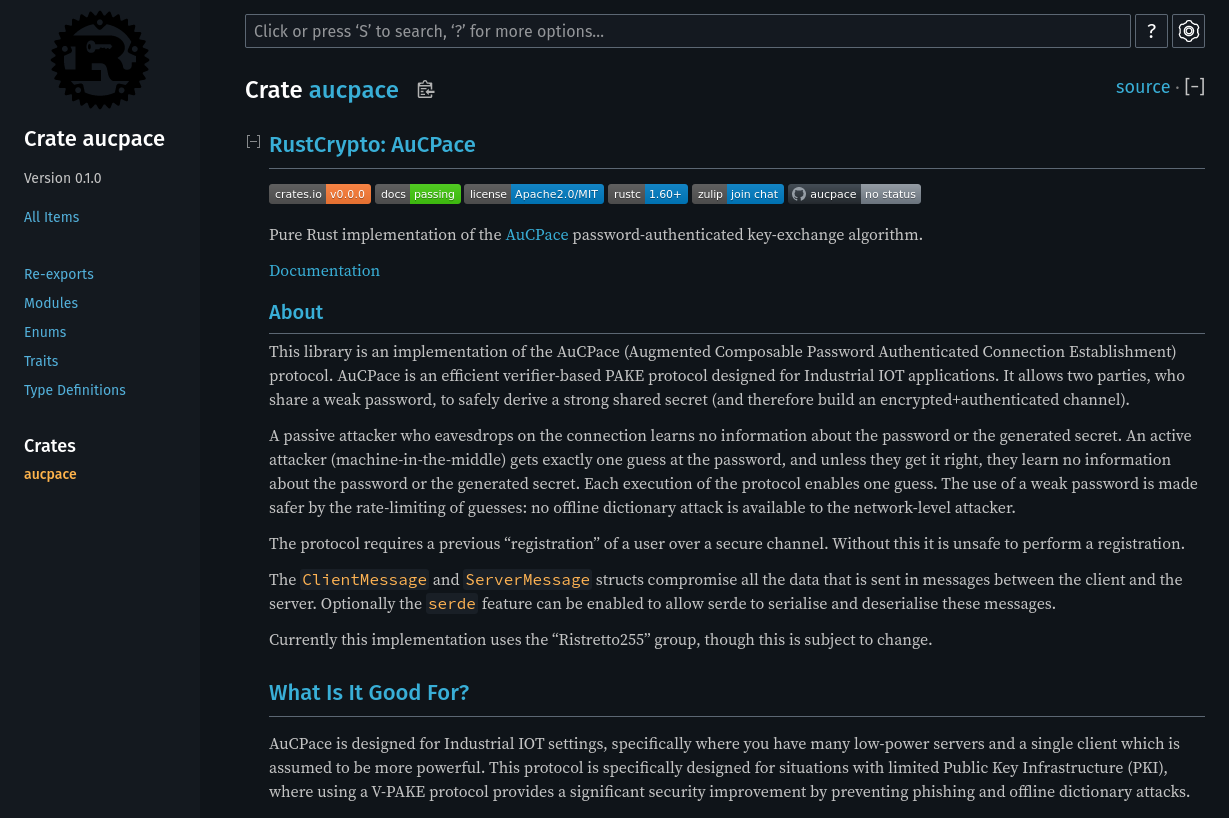
\includegraphics[width=\linewidth]{docs_front_page.png}
  \caption{Main Documentation Page}
  \label{fig:main-doc-page}
\end{figure}

\begin{figure}[H]
  \centering

  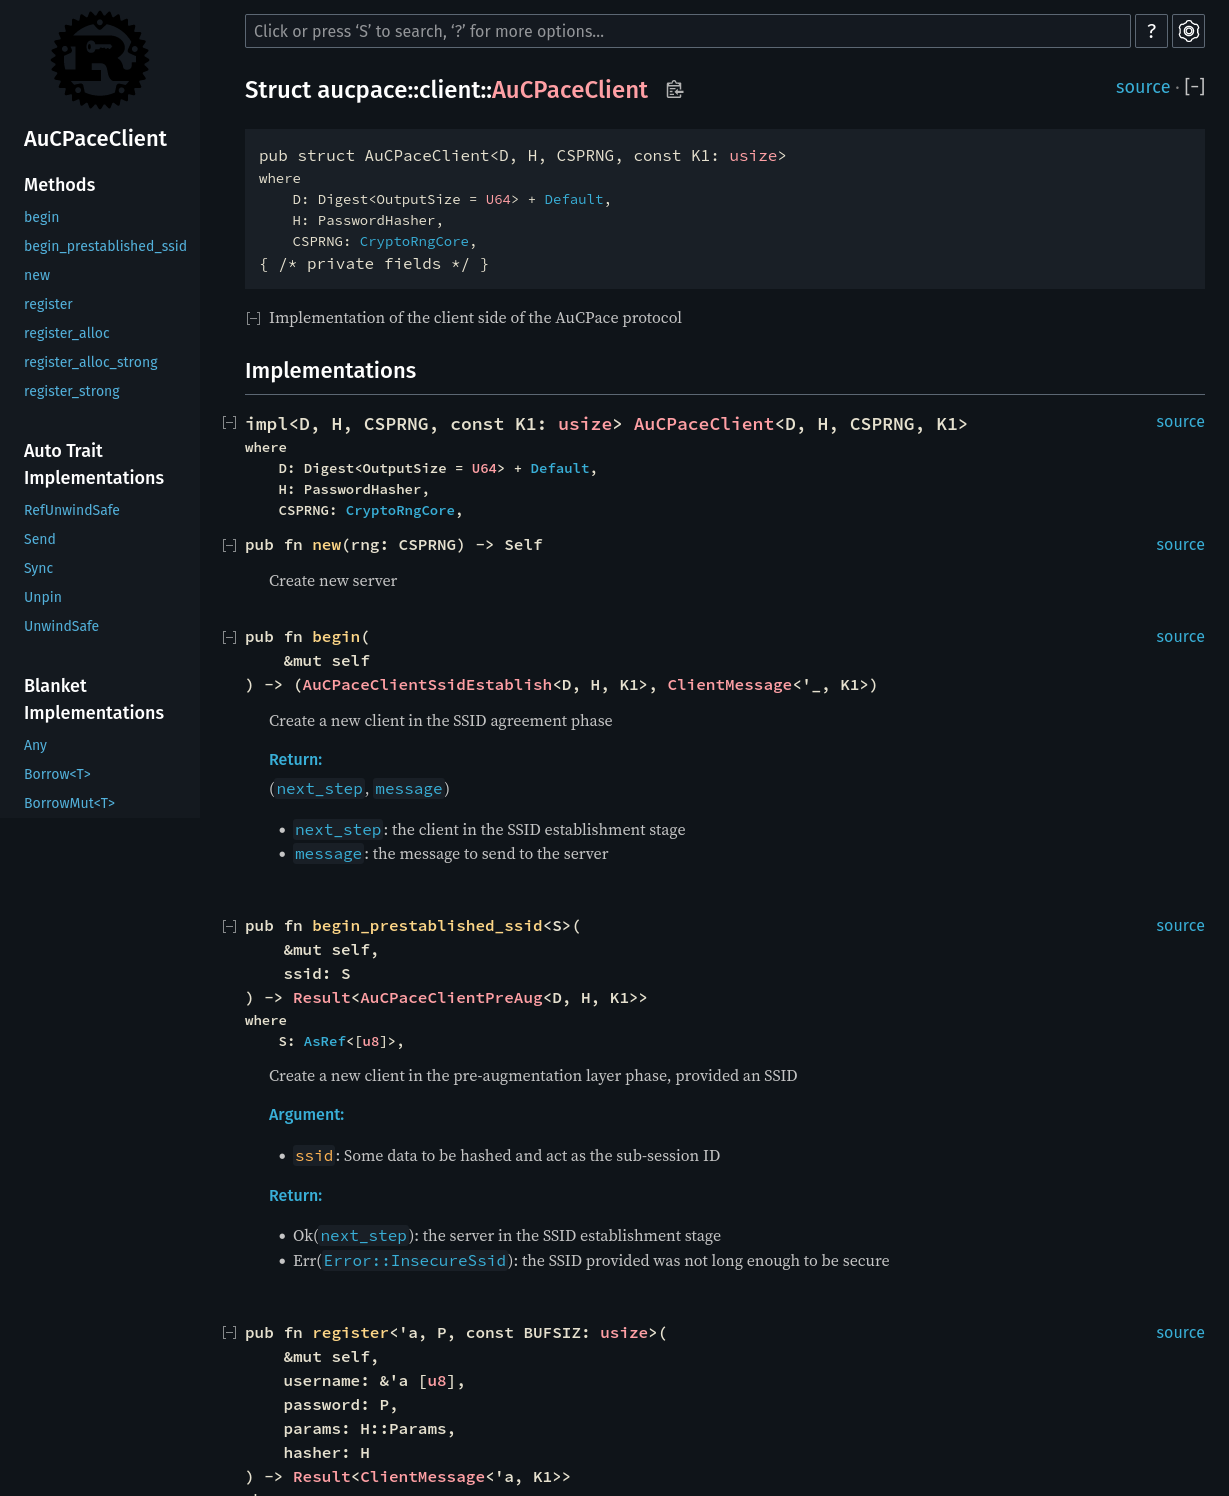
\includegraphics[width=\linewidth]{docs_aucpace_client.png}
  \caption{\texttt{AuCPaceClient} Documentation}
  \label{fig:aucpace-client-doc-page}
\end{figure}
